\appendix

\section{Examples of Checks and validations}
\seclabel{ChecksAndValidations}

All the results of the checking and the validation of the program is shown in one integrated view, it is called \emph{Problems}. The figure \figref{problemsview.png} shows a view of this feature. 
There are different types of problems, because these checks and validations are not only used to show type errors or syntax errors, but also to encourage some properties of the program we consider as main topics in the learning process of an OO language.

Here there is a list of all the validations and checking the tool is performing, and a brief reason why they are useful in the teaching of an object oriented language.

Todos los checkeos y problemas
generados se muestran agrupados en una vista dedicada a tal fín (Problems).

% En lo que sigue fui comentando las cosas que ya están dichas pero no quiero borrar esta enumeración porque está muy buena.
\begin{itemize}
   \item \textbf{De sintaxis}: dados por el parser y lexer automáticamente.
  \item \textbf{De estilo}: para promover uniformidad y consistencia de código.
  Ejemplos:
  		\begin{itemize}
  			\item \textit{Nombres}: variables camelcase comenzando en minúscula,
  			nombres de clases camelcase iniciando mayúscula, packages en minúsculas, etc.
  			\item \textit{Orden y agrupamiento}: dentro de un objeto o clase, primero
  			se definen sus referencias internas, luego constructores y finalmente los métodos.
  			\item \textit{Separación de programas}: las clases sólo se pueden definir
  			en archivos de tipo \textit{librería}, no dentro de un \textit{program}.
  			\item \textit{Evitar referencias duplicadas}: no se puede definir una
  			referencia con nombre ya utilizado en alguna otra referencia del contexto (local, método,
  			clase/objeto, etc.). Ni tampoco si ya está definida en la superclase.
		\end{itemize}
  \item \textbf{De resolución de referencias}: para evitar referencias a
  variables inexistentes y, en la medida de lo posible (por ser de tipado
  implícito) de envío de mensajes. Ejemplos:
  		\begin{itemize}
		  \item \textit{Referencias inexistentes}: a variables locales, parámetros, o
		  internas (clase/objeto).
		  \item \textit{Constructores inexistentes}: evaluando existencia de la
		  clase, y compatibilidad en el número de paråmetros.
		  \item \textit{Envío de mensajes (a this)}: al ser a this se pueden realizar
		  checkeos por la existencia del método y compatibilidad de parámetros, incluso sin
		  involucrar al sistema de tipos.
		\end{itemize}
  \item \textbf{De uso de referencias}: para la detección de código
  	erroneo o bien desactualizado. Por ejemplo: warnings por referencias nunca
 	utilizadas, nunca asignadas, o utilización de variables en lugar de valores.
  \item \textbf{De estructura}: evitan por ejemplo inconsistencias en las
  estructuras creadas por el alumno. Por ejemplo, se checkea
  que un método marcado como \textit{override} efectivamente esté
	sobrescribiendo.
  \item \textbf{De tipos}: verifican compatibilidad de referencias en base a sus
  tipos. Por ejemplo ante envío de mensajes, o asignaciones de variables. Basado
  en el sistema de tipos.
\end{itemize}


\section{Implementation}
\label{sec:implementation}
\np{Qué podemos decir de esto}

\section{Images}
Imágenes y otros detalles de wollok que no entran en las 6/7 páginas del artículo

	\begin{figure}[p]
	    \centering
		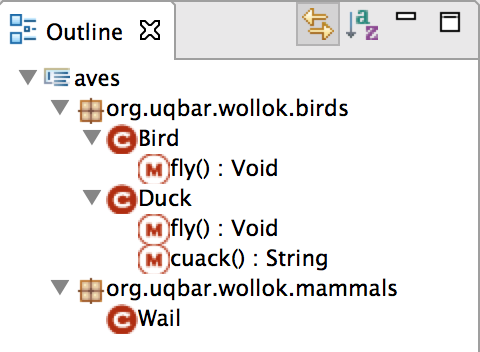
\includegraphics[scale=0.5]{images/wollok-paper-outline.png}
	    \caption{Outline View: muestra un resumen del contenido del archivo}
	    \label{fig:outline.png}
	\end{figure}
	
	\begin{figure}[p]
	    \centering
		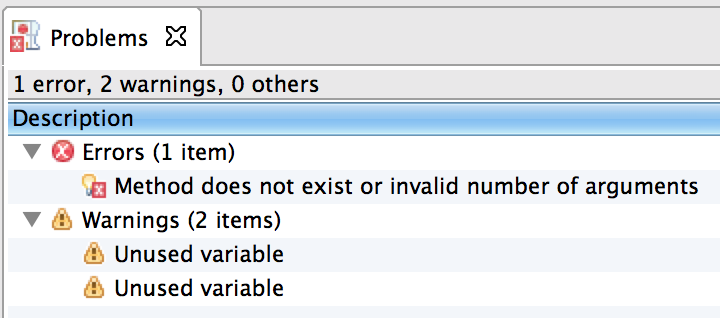
\includegraphics[scale=0.5]{images/wollok-paper-check-problemsview.png}
	    \caption{Vista de Problemas: errores y warnings}
	    \label{fig:problemsview.png}
	\end{figure}
	
	\begin{figure}[p]
	    \centering
		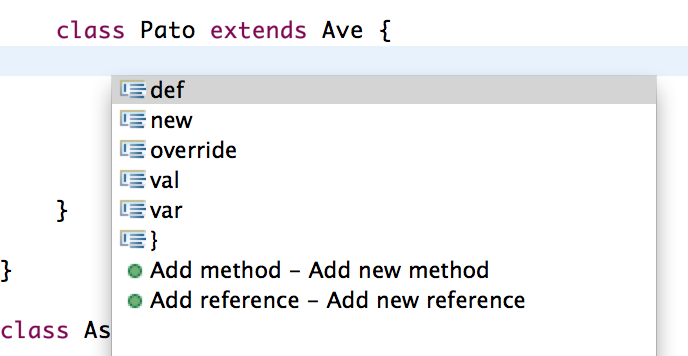
\includegraphics[scale=0.5]{images/wollok-paper-codetemplates.png}
	    \caption{Code Assist: templates para crear código rápidamente}
	    \label{fig:codetemplates.png}
	\end{figure}

	\begin{figure}[p]
	    \centering
		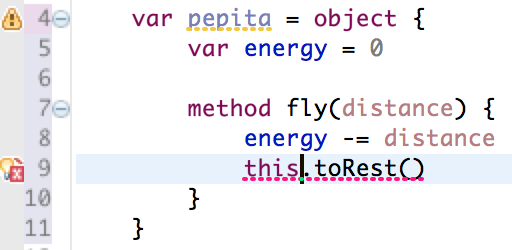
\includegraphics[scale=0.5]{images/wollok-paper-check-noMethodOnThis.png}
	    \caption{Checkeo de método inexistente en this}
	    \label{fig:check-noMethodOnThis.png}
	\end{figure}


\end{document}
